%%%%%%%%%%%%%%%%%%%%%%%%%%%%%%%%%%%%%%%%%
% Journal Article
% LaTeX Template
% Version 1.4 (15/5/16)
%
% This template has been downloaded from:
% http://www.LaTeXTemplates.com
%
% Original author:
% Frits Wenneker (http://www.howtotex.com) with extensive modifications by
% Vel (vel@LaTeXTemplates.com)
%
% License:
% CC BY-NC-SA 3.0 (http://creativecommons.org/licenses/by-nc-sa/3.0/)
%
%%%%%%%%%%%%%%%%%%%%%%%%%%%%%%%%%%%%%%%%%

%----------------------------------------------------------------------------------------
%	PACKAGES AND OTHER DOCUMENT CONFIGURATIONS
%----------------------------------------------------------------------------------------

\documentclass[twoside,twocolumn]{article}

\usepackage{blindtext} % Package to generate dummy text throughout this template 

\usepackage[sc]{mathpazo} % Use the Palatino font
\usepackage[T1]{fontenc} % Use 8-bit encoding that has 256 glyphs
\linespread{1.05} % Line spacing - Palatino needs more space between lines
\usepackage{microtype} % Slightly tweak font spacing for aesthetics

\usepackage[english,ngerman]{babel} % Language hyphenation and typographical rules

\usepackage[hmarginratio=1:1,top=32mm,columnsep=20pt]{geometry} % Document margins
\usepackage[hang, small,labelfont=bf,up,textfont=it,up]{caption} % Custom captions under/above floats in tables or figures
\usepackage{booktabs} % Horizontal rules in tables

\usepackage{lettrine} % The lettrine is the first enlarged letter at the beginning of the text

\usepackage{enumitem} % Customized lists
\setlist[itemize]{noitemsep} % Make itemize lists more compact

\usepackage{abstract} % Allows abstract customization
\renewcommand{\abstractnamefont}{\normalfont\bfseries} % Set the "Abstract" text to bold
\renewcommand{\abstracttextfont}{\normalfont\small\itshape} % Set the abstract itself to small italic text

\usepackage{titlesec} % Allows customization of titles
\renewcommand\thesection{\Roman{section}} % Roman numerals for the sections
\renewcommand\thesubsection{\roman{subsection}} % roman numerals for subsections
\titleformat{\section}[block]{\large\scshape\centering}{\thesection.}{1em}{} % Change the look of the section titles
\titleformat{\subsection}[block]{\large}{\thesubsection.}{1em}{} % Change the look of the section titles

\usepackage{fancyhdr} % Headers and footers
\pagestyle{fancy} % All pages have headers and footers
\fancyhead{} % Blank out the default header
\fancyfoot{} % Blank out the default footer
\fancyhead[C]{QC Optimization Challenge $\bullet$ QAR-Lab, LMU München $\bullet$ TRUMPF $\bullet$ 15. Juli 2021} % Custom header text
\fancyfoot[RO,LE]{\thepage} % Custom footer text

\usepackage{titling} % Customizing the title section

\usepackage{hyperref} % For hyperlinks in the PDF

\usepackage{url}
\usepackage{grffile}

\usepackage{subcaption}
\usepackage{floatrow}
\usepackage{graphicx}
\usepackage{float}
\usepackage{wrapfig}

%----------------------------------------------------------------------------------------
%	TITLE SECTION
%----------------------------------------------------------------------------------------

\setlength{\droptitle}{-4\baselineskip} % Move the title up

\pretitle{\begin{center}\Huge\bfseries} % Article title formatting
\posttitle{\end{center}} % Article title closing formatting
\title{Projektbericht \\QC Optimization Challenge} % Article title
\author{%
\textsc{Ege Çimşir, Jonas Gottal, Sebastian Silva, Tobias Rohe, Viktoria Patapovich}\\[1ex] % Your name
\normalsize Ein Projekt des QAR-Lab der LMU München mit TRUMPF in Kooperation mit \\\normalsize PlanQK und dem QAR-Lab Bayern\thanks{Weitere Informationen unter \url{mobile.ifi.lmu.de/lehrveranstaltungen/praktikum-qcp-sose2021/}} % Your institution
%\normalsize \href{mailto:john@smith.com}{john@smith.com} % Your email address
%\and % Uncomment if 2 authors are required, duplicate these 4 lines if more
%\textsc{Jane Smith}\thanks{Corresponding author} \\[1ex] % Second author's name
%\normalsize University of Utah \\ % Second author's institution
%\normalsize \href{mailto:jane@smith.com}{jane@smith.com} % Second author's email address
}
\date{15. Juli 2021} % Leave empty to omit a date
\renewcommand{\maketitlehookd}{%
\begin{abstract}
\noindent Das Job-Shop-Scheduling Problem gehört zu der Komplexitätsklasse NP-hart und beschäftigt gleichermaßen Wissenschaft wie Industrie. Im Rahmen der QC-Optimization-Challenge hat die Firma TRUMPF eine Erweiterung dieser Problemstellung geboten. Hierbei geht es sowohl um die zeitliche Planung als auch Zuweisung verschiedener Bauteile auf eine Reihe von Maschinen. Zur Lösung dieses Problems stehen mehrere Quantencomputer zur Verfügung, welche sich in zwei Quantum Annealer und zwei Quantum Gate Model-Computer unterteilen lassen. Die folgende Ausarbeitung zeigt, dass bisher lediglich hybride Annealing-Ansätze solche industrienahen Problemstellungen bewältigen können.
\end{abstract}
}

%----------------------------------------------------------------------------------------

\begin{document}

% Print the title
\maketitle

%----------------------------------------------------------------------------------------
%	ARTICLE CONTENTS
%----------------------------------------------------------------------------------------

\section{Einleitung}

\lettrine[nindent=0em,lines=3]{O}bwohl Quantencomputer in aller Munde sind, bleibt doch ihre Funktionsweise und ihre aktuellen Fähigkeiten für viele im Verborgenen. Die wichtigste Frage für die Wirtschaft ist daher: Wann und wo kann ein Quantencomputer gewinnbringend eingesetzt werden? Wir haben in unserer Arbeit das flexible Job-Shop-Scheduling-Problem (JSSP) modelliert und auf echter Quantenhardware getestet. Unser Fokus lag speziell auf dem Vergleich der Ansätze \textit{Quantum Annealing} und \textit{Quantum Gate Model}, sowie deren aktuelle praktische Relevanz. Des Weiteren kann aus unserer Arbeit der Workflow der Modellierung bis hin zur Ausführung auf einer Quantum Processing Unit (QPU) nachvollzogen werden. Im Nachfolgenden Teil werden das Konzept vorgestellt und die Ergebnisse beider Ansätze beschrieben und verglichen.


%------------------------------------------------

\section{Konzept}
Unsere Aufgabe für die \textit{QC-Optimization-Challenge} des \textit{QAR-Lab} wurde von dem Unternehmen TRUMPF bereitgestellt: Für aus Rohblechen geschnittene Kleinteile muss zur Weiterverarbeitung eine richtige und effiziente Maschinenbelegung gefunden werden ohne eine Deadline zu überschreiten. Da Quantencomputer im allgemeinen die beste Lösung anhand ihres Energielevels suchen, müssen wir unser Problem neu formulieren: \textit{Quadratic Unconstrained Binary Optimization}, kurz QUBO, ist eine Form zur Beschreibung NP-harter kombinatorischer Optimierungsprobleme. Sie besteht meist aus einer zu minimierenden Kostenfunktion sowie Straftermen, welche dazu dienen Felder in der QUBO-Matrix für den Quantencomputer energetisch teuerer und somit uninteressanter zu machen. Bevor wir diese mit einem Quantencomputer lösen, haben wir unsere Variablen mithilfe diverser Pruning Methoden stark reduziert und zur besseren Vergleichbarkeit der Ergebnisse einzelne Jobsets für diverse Komplexitätsklassen definiert.


%------------------------------------------------

\section{Ergebnisse}
\textsc{Annealing:} Die beiden Annealer D-Wave Advantage und Fujitsu DAU haben wir unter dem Gesichtspunkt des globalen Energieminimums (Optimum) -- einer \textit{Best Known Solution (BKS)}, also einem Ergebnis, bei dem weder Strafterme noch Kostenfunktion verletzt wurden -- verglichen. Außerdem definieren wir eine  \textit{Good Known Solution (GKS)} als ein Ergebnis bei dem maximal ein Zeitschritt über die Deadline verstrichen ist. 

\begin{figure}[H]
        \centering
        \begin{subfigure}[b]{0.49\textwidth}
            \centering
            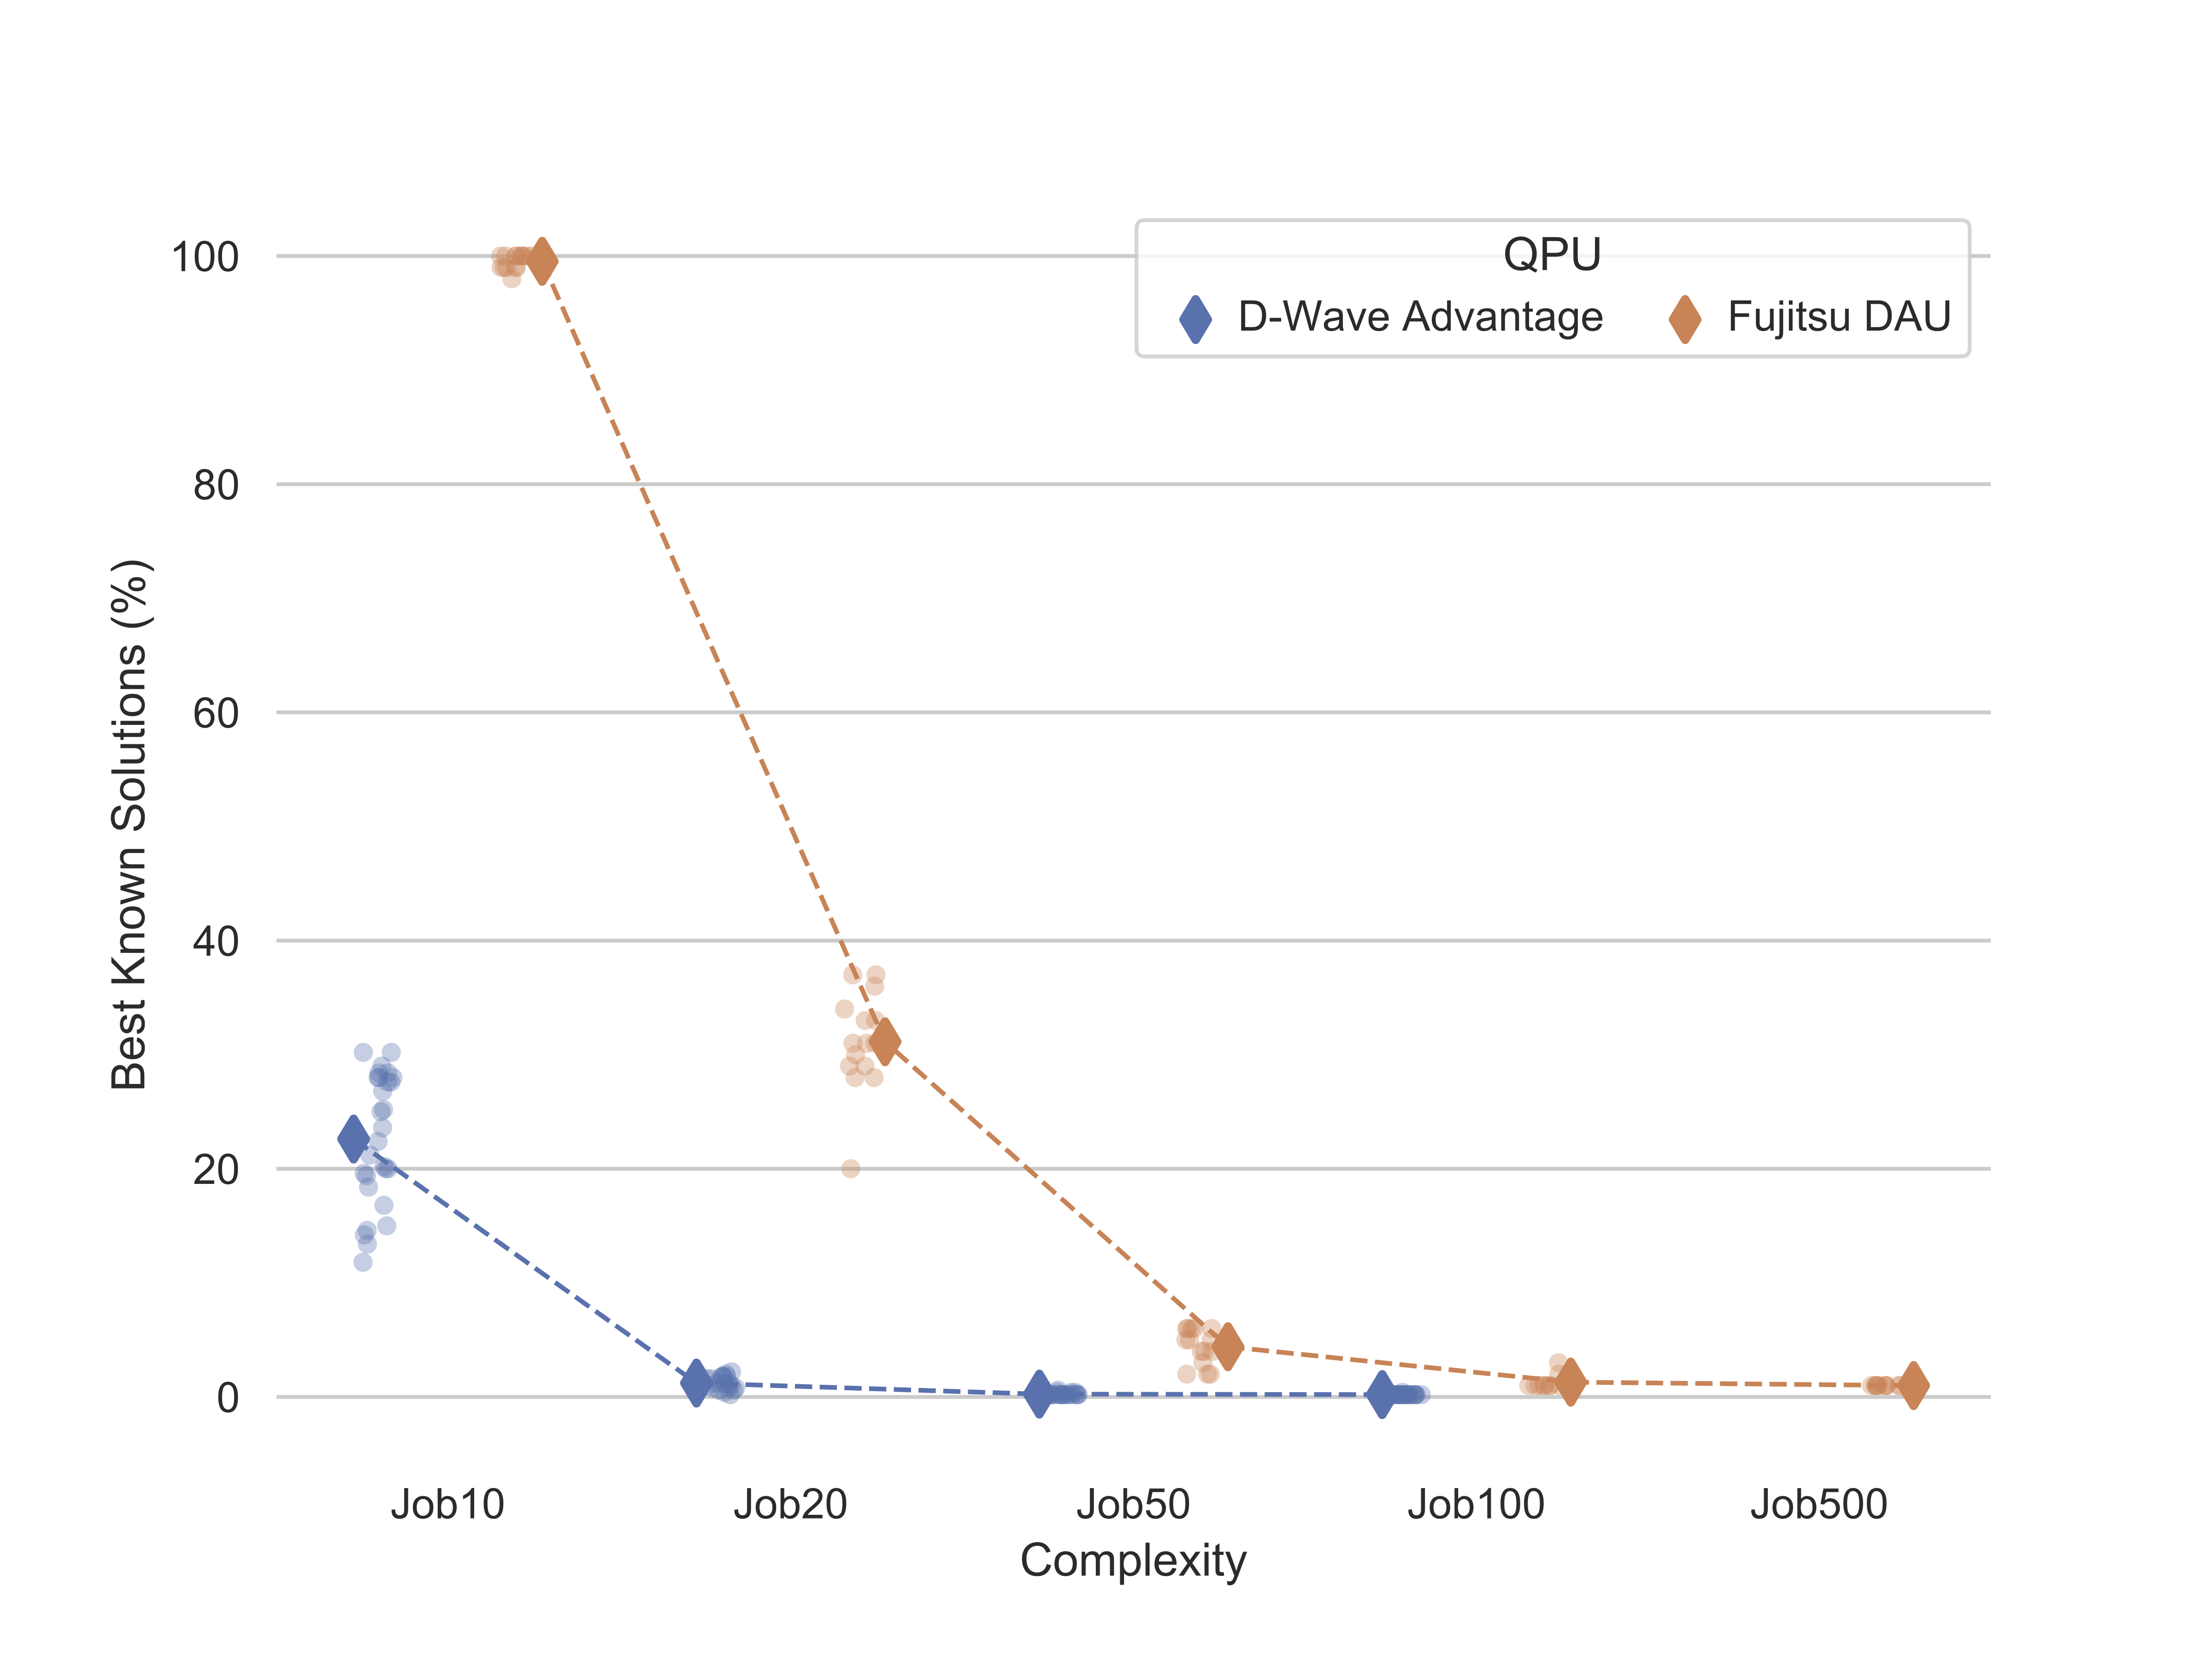
\includegraphics[trim={0.75cm 0.5cm 1.25cm 1.7cm}, clip,width=\textwidth]{images/Best Known Solutions by Complexity.png}
            \caption[]%
            {{\small BKS (\%)}}    
            \label{fig:BKS}
        \end{subfigure}
        \begin{subfigure}[b]{0.49\textwidth}  
            \centering 
            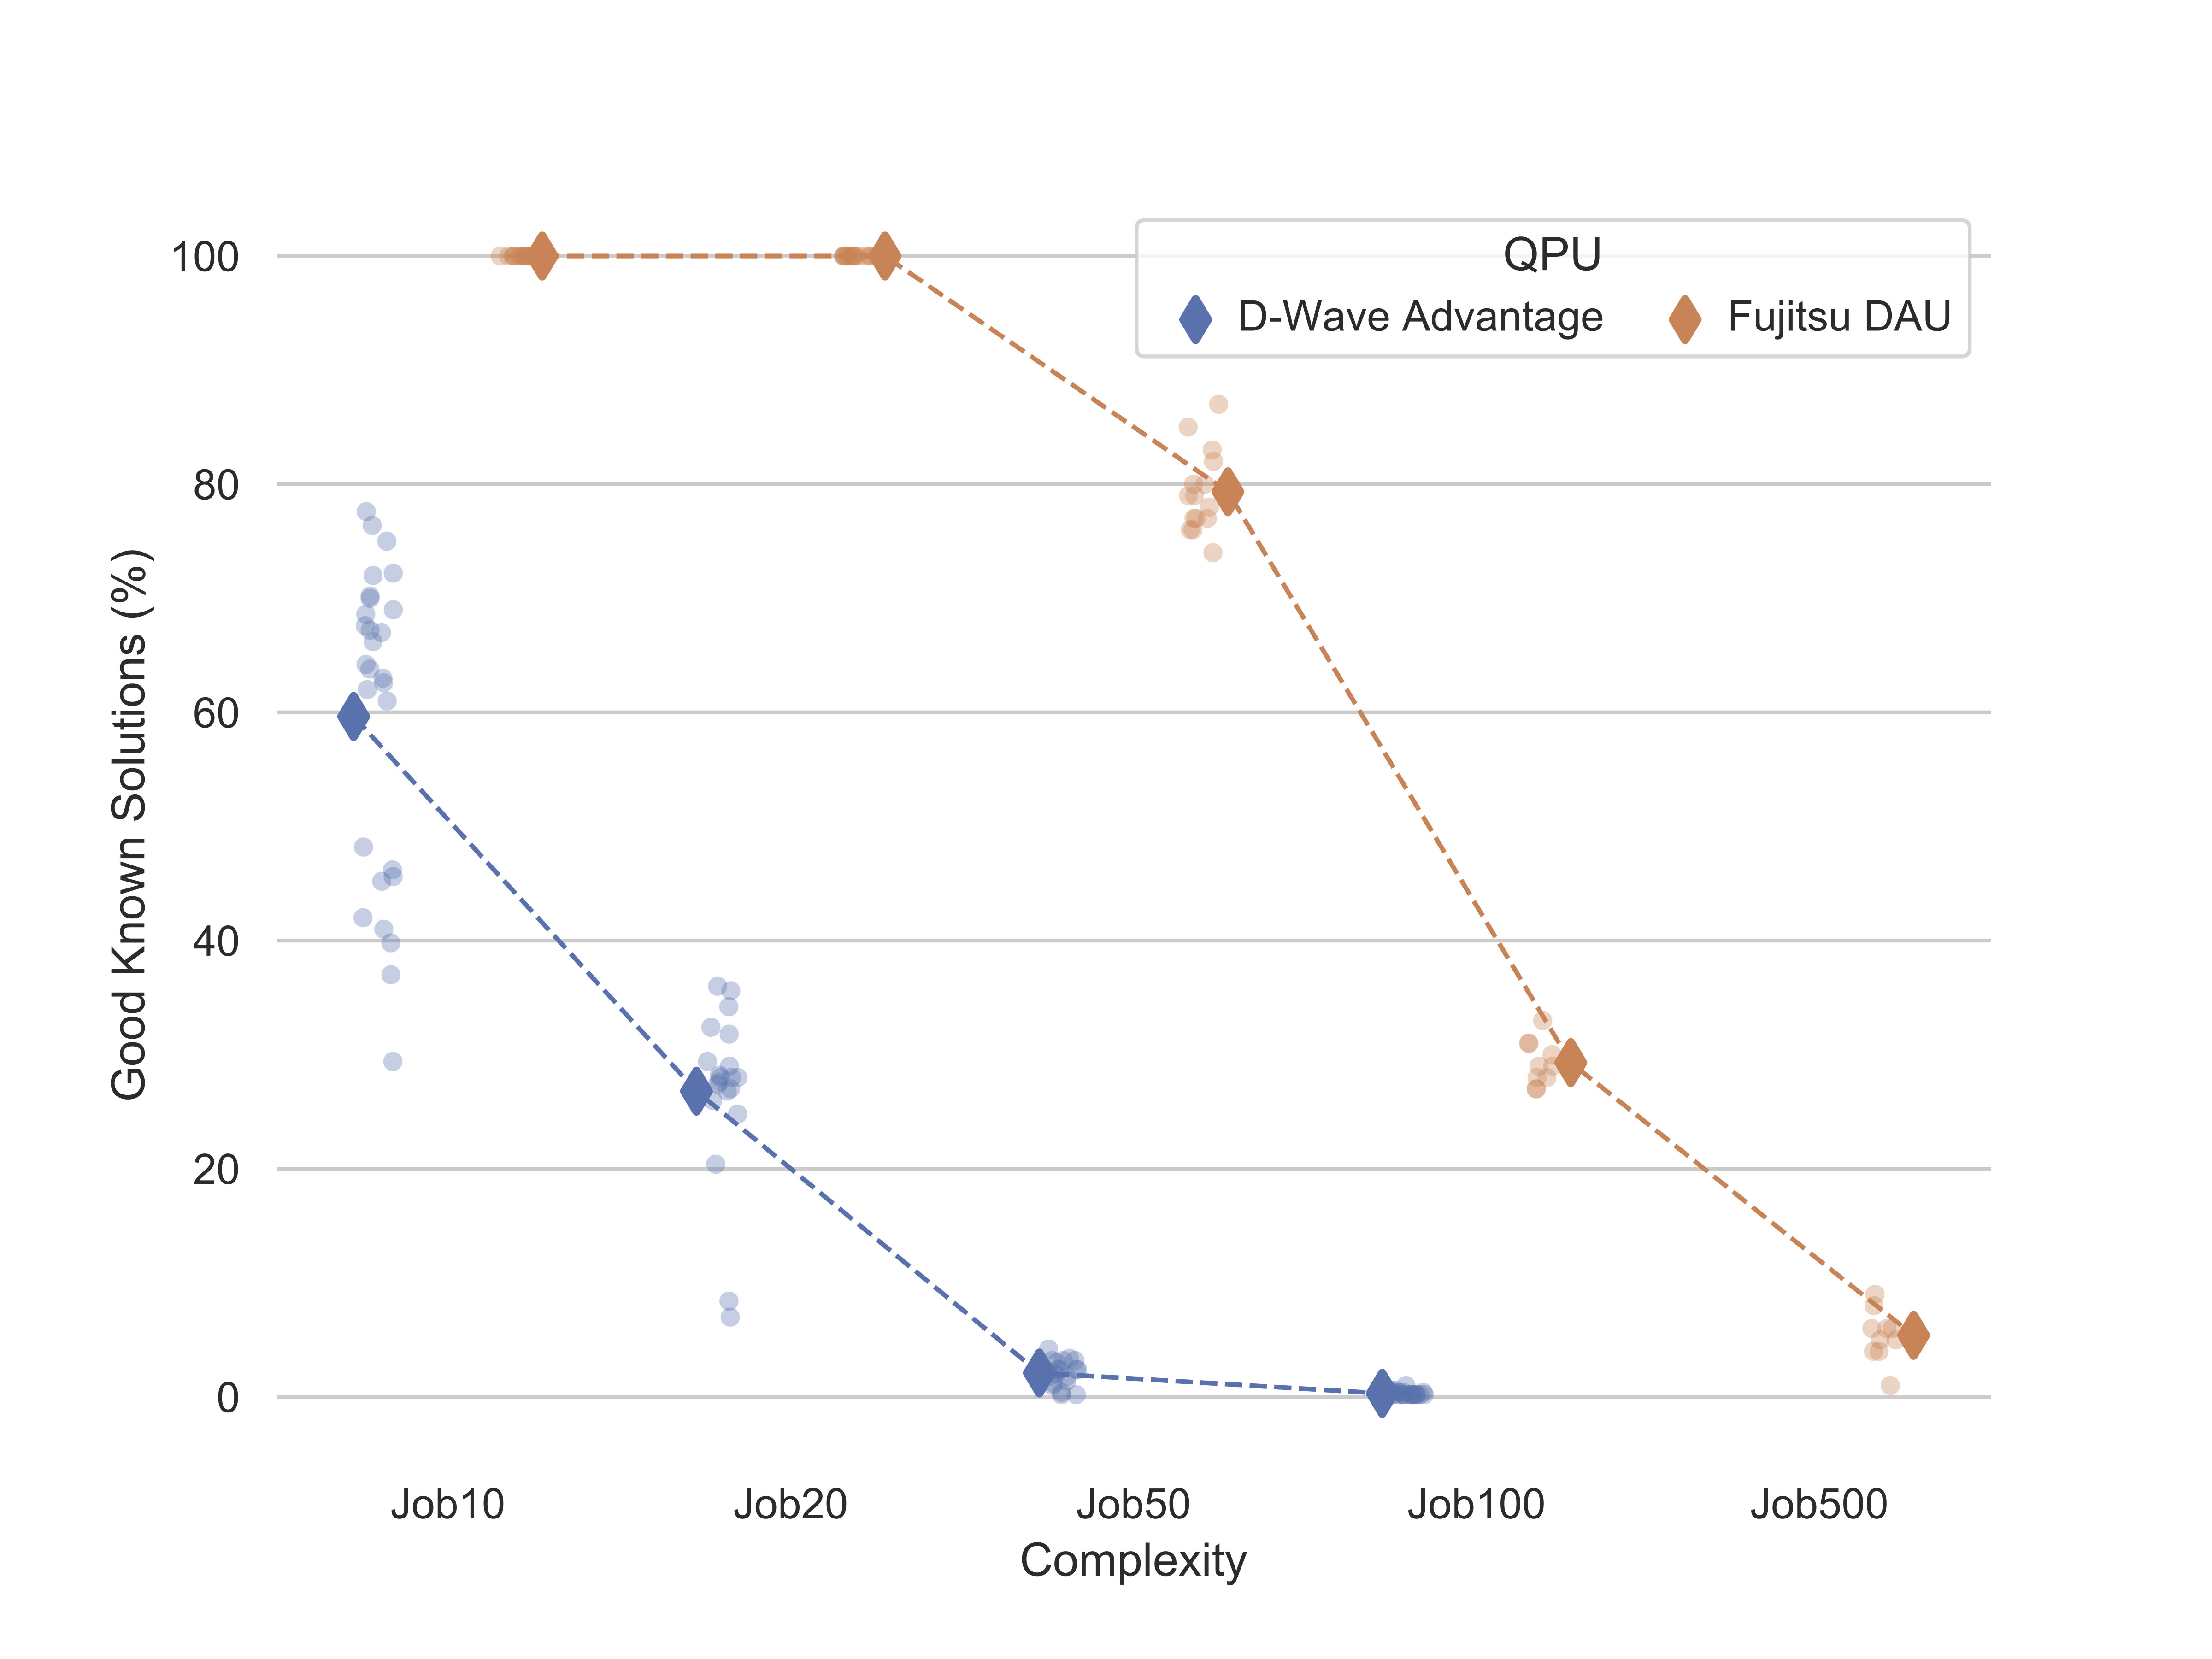
\includegraphics[trim={0.75cm 0.5cm 1.25cm 1.7cm}, clip,width=\textwidth]{images/Good Known Solutions by Complexity.png}
            \caption[]%
            {{\small GKS (\%)}}    
            \label{fig:GKS}
        \end{subfigure}
        \caption[ Ergebnisse nach Komplexität ]
         {\small Ergebnisse nach Komplexität} 
        \label{fig:A}
    \end{figure}
    \vspace{-15pt}
\begin{figure}[H]
        \centering
        \begin{subfigure}[b]{0.49\textwidth}
            \centering
            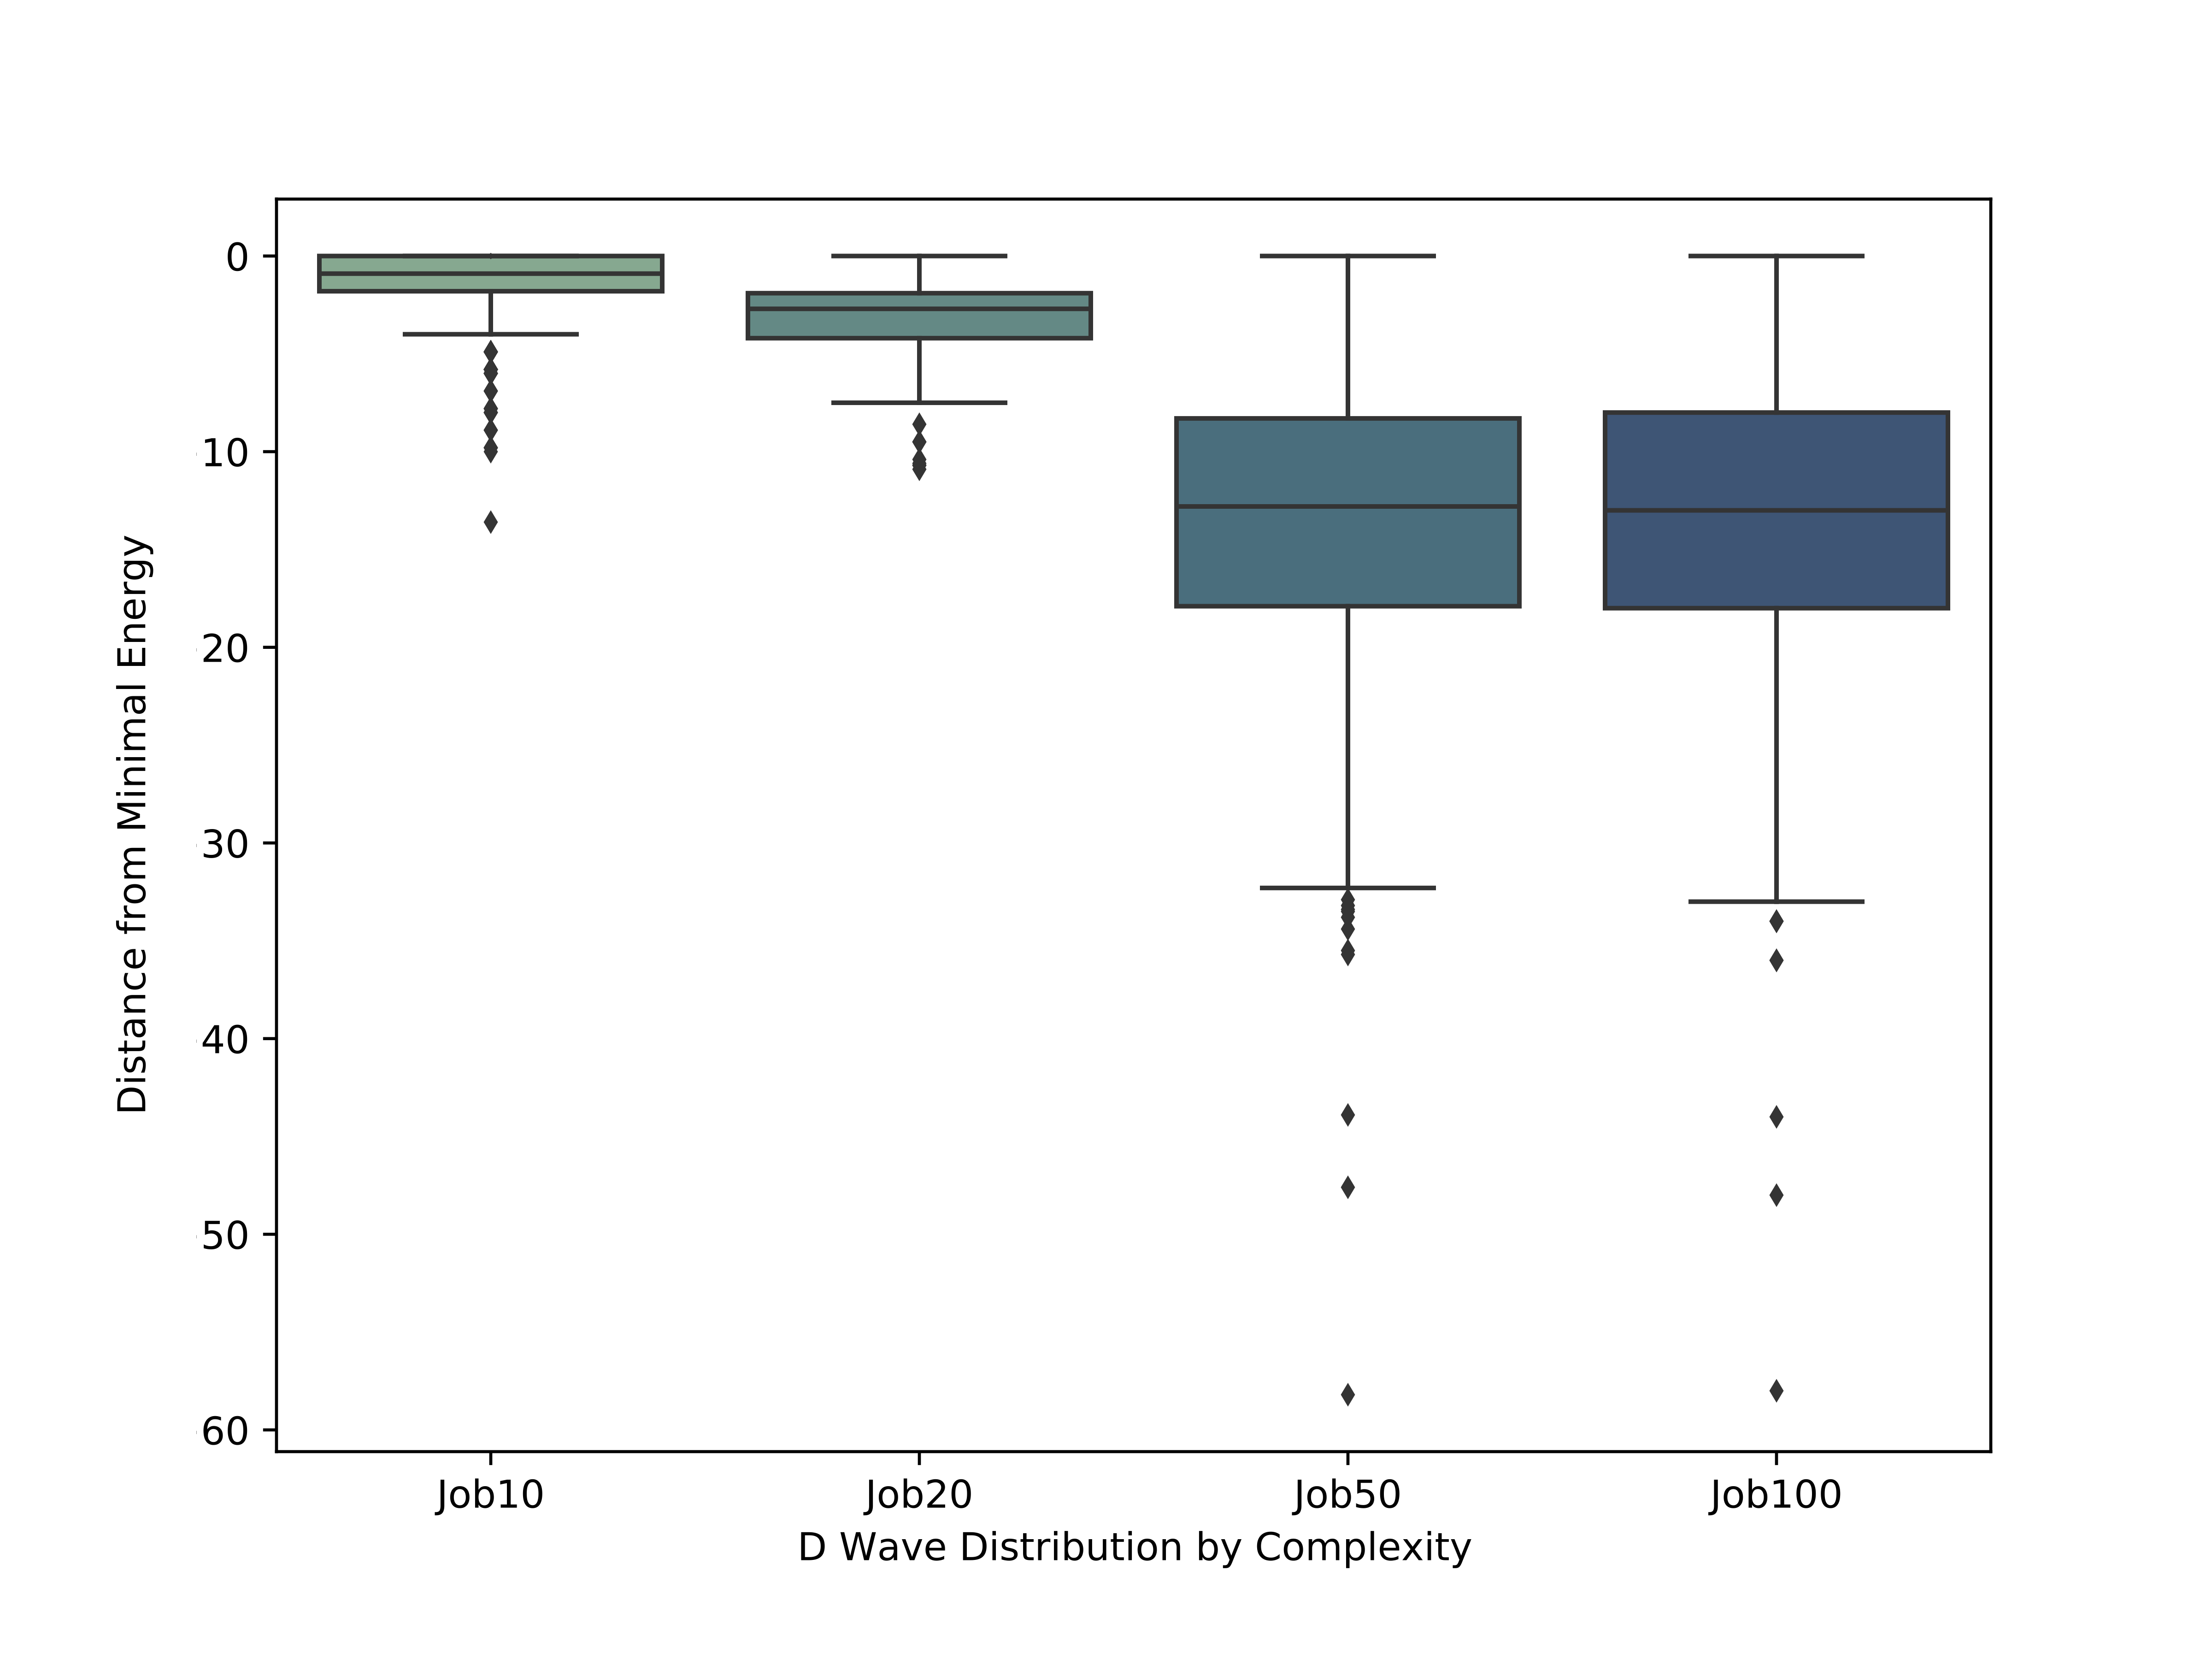
\includegraphics[trim={0 0.7cm 0 1.7cm}, clip,width=\textwidth]{images/D Wave Deviation.png}
            \caption[]%
            {{\small D-Wave  }}    
            \label{fig:DeviationDWave}
        \end{subfigure}
        \begin{subfigure}[b]{0.49\textwidth}  
            \centering 
            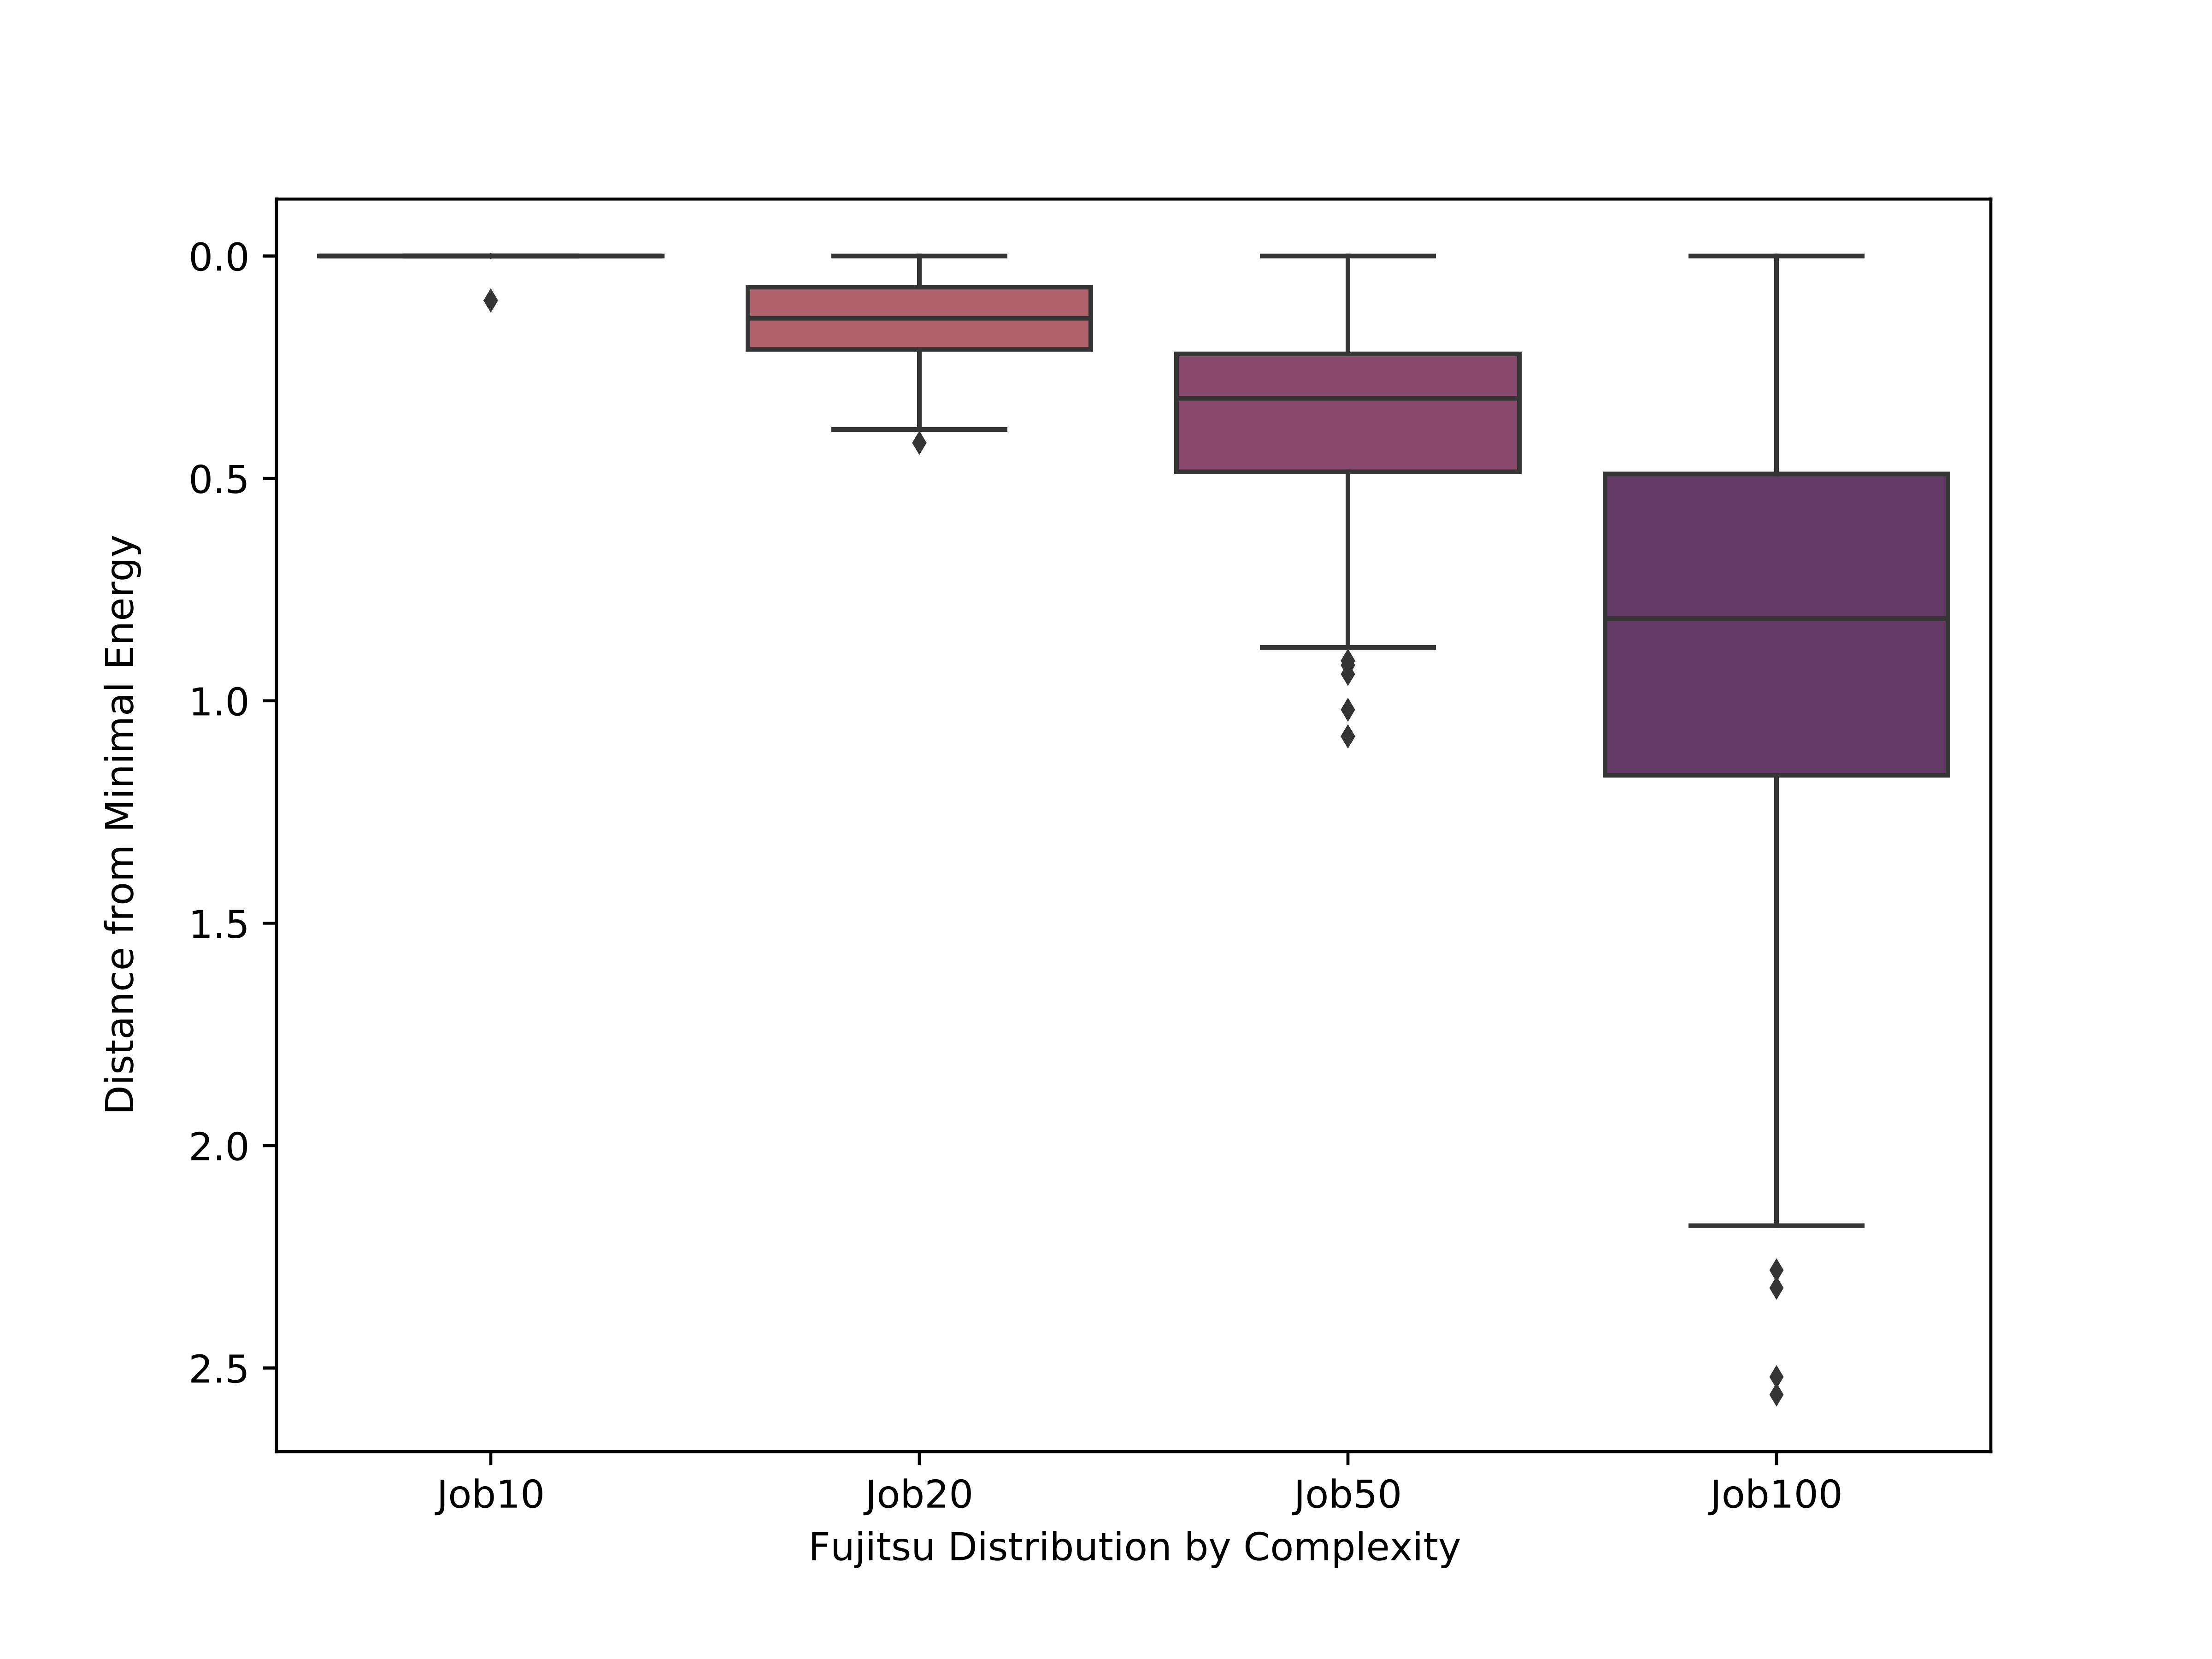
\includegraphics[trim={0 0.7cm 0 1.7cm}, clip,width=\textwidth]{images/Fujitsu Deviation.png}
            \caption[]%
            {{\small Fujitsu }}    
            \label{fig:DeviationFujitsu}
        \end{subfigure}
        \caption[ Ergebnisse nach Komplexität ]
         {\small  Abweichungen vom Optimum ( $\widehat{=}~0$ ) } 
        \label{fig:B}
    \end{figure}
  \vspace{-5pt}

Wie man an Abbildung \ref{fig:A} erkennt, sind die QPU Solver der aktuellen Generation noch nicht leistungsstark genug, um unsere größeren Problemstellungen anzugehen. Desweiteren erkennt man in Abbildung \ref{fig:B}, dass das Streuverhalten der Quantum-Annealer zu keinen zuverlässigen Ergebnissen bei mittleren Problemen führt. Daher haben wir uns zusätzlich mit den folgenden hybriden Ansätzen auseinander gesetzt: Die Komplettlösung \textit{D-Wave Leap} -- eine Kombination aus Decomposer und QPU als Solver -- die aber nur eine finale Lösung zurück gibt und wenig Einblick in die Funktionsweise bietet. Sowie die Kombination aus Qbsolv als Decomposer mit dem D-Wave Advantage als QPU. Qbsolv zerlegt dabei die QUBO in kleinere Teil-Probleme (Sub-QUBOs), die dann unabhängig voneinander von der QPU gelöst werden. Beide Ansätze lieferten auch für komplexe Probleme zuverlässig valide Lösungen. Der Mehrwert der QPU in dieser Konstellation bleibt jedoch noch aus.\\\\
\textsc{Gate Model:} Auch wenn der Ansatz des Quantum Gate Models äußerst vielversprechend ist, so kann er aktuell seinen hohen Erwartungen leider nicht gerecht werden. Beide getesteten Quantencomputer, IBM Quantum System-One und Rigetti Aspen-9, konnten selbst für äußerst kleine Jobsets mit lediglich zwei einfachen Jobs die optimale Belegung nicht finden. 
Nach wie vor dominiert das sog. Quantenrauschen alle Ergebnisse. Des Weiteren haben wir in unserer Arbeit zwei verschiedene Ansätze der Parameteroptimierung angewandt. Zum einen wurden die Parameter sowohl auf einer klassischen CPU voroptimiert als auch auf der QPU nachoptimiert, im anderen Fall lediglich voroptimiert.
Es muss jedoch erwähnt werden, dass das Ergebnis von IBM bei einfacher Optimierung, das richtige Ergebnis zumindest am zweithäufigsten zurückgibt. Besonders interessant sind die Tatsachen, dass die doppelt optimierten Parameter sowohl in Sachen Ausschlagsgröße der richtigen Lösung als auch Varianz der Ergebnisse merkbar schlechter abschneiden. Dies geht entgegen der Intuition, dass mehr Optimierung stets zu besseren Ergebnissen führt.
%------------------------------------------------

\section{Fazit}
Unsere Forschung soll dazu beitragen den aktuellen Stand des Quantencomputings näher zu beschreiben und Anhaltspunkte für die zukünftige Entwicklung zu geben. Ob die Versprechungen dieser neuen Technologie letztendlich eingehalten werden und ein gewaltiger Technologiesprung erreicht werden kann, kann nach wie vor nicht mit Sicherheit vorhergesagt werden.  Was allerdings sicher erscheint ist, dass dieses Feld hoch dynamisch bleibt und viele Überraschungen bereithält. 



%----------------------------------------------------------------------------------------
%	REFERENCE LIST
%----------------------------------------------------------------------------------------

%\bibliography{references}
%\bibliographystyle{plain}

%----------------------------------------------------------------------------------------

\end{document}
